\documentclass[journal]{IEEEtran}

\usepackage{booktabs}
\usepackage{placeins}
\usepackage{acronym}
\usepackage{amsmath,amssymb,amsfonts}
\usepackage{tabularx}
\usepackage{stfloats}
\usepackage{siunitx}
\usepackage{graphicx}
\usepackage{mathtools}
\usepackage{array}
\usepackage{url}
\usepackage{xspace}
\usepackage{cite}
\usepackage{threeparttable}
\usepackage{multirow}

\newcolumntype{L}[1]{>{\raggedright\arraybackslash}m{#1}}
\newcolumntype{C}[1]{>{\centering\arraybackslash}m{#1}}

\acrodef{MRI}{magnetic resonance imaging}
\acrodef{T2W}{T2-weighted}
\acrodef{DWI}{diffusion-weighted imaging}
\acrodef{CNN}{convolutional neural network}
\acrodef{CVNN}{complex-valued neural network}
\acrodef{RVNN}{real-valued neural network}
\acrodef{PI-RADS}{Prostate Imaging Reporting and Data System}
\acrodef{FFT}{fast Fourier transform}
\acrodef{RSS}{root-sum-of-squares}
\acrodef{RMS}{root-mean-square}
\acrodef{BN}{batch normalization}
\acrodef{AUC}{area under the receiver operating characteristic curve}
\acrodef{ROC}{receiver operating characteristic}
\acrodef{AP}{average precision}
\acrodef{BCE}{binary cross entropy}
\acrodef{GRAPPA}{generalized autocalibrating partially parallel acquisitions}
\acrodef{ACS}{autocalibration signal}
\acrodef{CI}{confidence interval}
\acrodef{WL}{widely linear}

% Generated by report/scripts/analyze_results.py; do not edit by hand.
% All scalar values are regenerated from results/test_metrics_all_runs.csv.
\newcommand{\ComplexTotal}{480\xspace}
\newcommand{\RealAUC}{0.7268\xspace}
\newcommand{\RealAP}{0.1063\xspace}
\newcommand{\ImageAUC}{0.7102\xspace}
\newcommand{\ImageAP}{0.1189\xspace}
\newcommand{\FourierAUC}{0.6377\xspace}
\newcommand{\FourierAP}{0.0920\xspace}
\newcommand{\ComplexMeanAUC}{0.6740\xspace}
\newcommand{\ComplexMeanAP}{0.1055\xspace}
\newcommand{\ComplexMinAUC}{0.3464\xspace}
\newcommand{\BestAUC}{0.8162\xspace}
\newcommand{\BestAP}{0.1655\xspace}
\newcommand{\BestLabel}{cx\_img\_med\_cbn\_std\_single\_holo\_card\xspace}
\newcommand{\ComplexWins}{130\xspace}
\newcommand{\CanonicalMaxAUC}{0.7527\xspace}
\newcommand{\CanonicalMedianAUC}{0.7283\xspace}
\newcommand{\CanonicalAverageAUC}{0.7156\xspace}
\newcommand{\FourierBatchnormAUC}{0.6448\xspace}
\newcommand{\FourierRmsAUC}{0.6306\xspace}
\newcommand{\ImageBatchnormAUC}{0.7252\xspace}
\newcommand{\ImageRmsAUC}{0.6953\xspace}
\newcommand{\ConvStandardAUC}{0.6771\xspace}
\newcommand{\ConvWidelyLinearAUC}{0.6709\xspace}
\newcommand{\ActCardioidAUC}{0.6714\xspace}
\newcommand{\ActCreluAUC}{0.6731\xspace}
\newcommand{\ActMagnitudeSiluAUC}{0.6712\xspace}
\newcommand{\ActModreluAUC}{0.6802\xspace}

% Generated by report/scripts/analyze_results.py; do not edit by hand.
\newcommand{\TopTableRows}{%
1 & cx\_img\_med\_cbn\_std\_single\_holo\_card & 0.8162 & 0.1655 & image / median / batchnorm / standard / cardioid / (complex\_only / holographic) \\
2 & cx\_img\_med\_cbn\_std\_single\_none\_card & 0.7971 & 0.1606 & image / median / batchnorm / standard / cardioid / (complex\_only / none) \\
3 & cx\_img\_max\_cbn\_std\_dual\_holo\_magsilu & 0.7920 & 0.1491 & image / max / batchnorm / standard / magnitude\_silu / (dual / holographic) \\
4 & cx\_img\_avg\_cbn\_std\_dual\_holo\_crelu & 0.7896 & 0.1795 & image / average / batchnorm / standard / crelu / (dual / holographic) \\
5 & cx\_img\_avg\_cbn\_wl\_dual\_gate\_card & 0.7893 & 0.2142 & image / average / batchnorm / widely\_linear / cardioid / (dual / modulus\_gate) \\
}


\begin{document}

\title{Complex-Valued Neural Networks for Prostate MRI Classification: A Parameter-Matched Factorial Study}

\author{Author names and affiliations to be supplied%
\thanks{Author list, affiliations, funding information, and corresponding-author details must be finalized before submission.}}

\markboth{AUTHOR \MakeLowercase{et al.}: Complex-Valued Neural Networks for Prostate MRI Classification}%
{Author \MakeLowercase{\emph{et al.}}}

\maketitle

\begin{abstract}
Magnetic resonance data are acquired as complex-valued signals, yet diagnostic learning pipelines commonly discard phase and operate on magnitude images. We study slice-level PI-RADS radiological-suspicion classification using prepared fastMRI Prostate T2-weighted MRI, comparing one fixed real magnitude CNN with 480 parameter-matched complex configurations. The factorial grid varies image-domain versus an FFT-derived Fourier-domain representation, pooling, normalization, convolution, activation, and a combined stream/interaction factor. All 481 reported runs use fixed seed 10383 and patient-disjoint training, validation, and test partitions. Because the positive class is strongly imbalanced, AUC is the main discrimination metric and average precision (AP) is reported as a complementary metric. The real baseline achieved AUC 0.7268, while only 130/480 complex configurations exceeded it. Mean AUC was 0.7102 in the image domain and 0.6377 in the Fourier domain; image-domain AUC was higher in 196/240 matched architecture pairs (81.7\%), with mean paired image-minus-Fourier AUC difference of +0.0725. The maximum observed AUC of 0.8162 is exploratory because the same fixed held-out test cohort was reused across configurations. The results support an architecture- and representation-dependent benefit of complex-valued processing rather than a universal advantage of complex arithmetic. The grid contains one training realization per architecture, so these conclusions characterize a fixed experimental surface rather than optimization variability or independently validated final-model performance.
\end{abstract}

\begin{IEEEkeywords}
Complex-valued neural networks, magnetic resonance imaging, prostate MRI, fastMRI, T2-weighted imaging, k-space, phase information, medical image classification.
\end{IEEEkeywords}

\IEEEpeerreviewmaketitle
\acresetall

% =============================================================================
\section{Introduction}\label{sec:introduction}
% =============================================================================
\IEEEPARstart{M}{agnetic} resonance imaging is intrinsically complex-valued. Receiver coils measure oscillating electromagnetic signals whose samples have real and imaginary components. Conventional image formation eventually produces magnitude images that are convenient for visualization and clinical interpretation, but the magnitude operation is many-to-one: different complex signals can map to the same nonnegative intensity. A diagnostic network trained only on magnitude therefore never receives the phase-bearing part of the acquisition, even when that information is present in the stored multicoil signal.

A complex sample $z=a+\mathrm{i}b=r\mathrm{e}^{\mathrm{i}\phi}$ jointly represents amplitude $r$ and phase $\phi$. Complex-valued processing is not merely a two-channel implementation choice. Complex multiplication constrains how the Cartesian components interact, global rotations have a natural group action, and several nonlinearities and pooling rules can be distinguished by whether they preserve, select, or explicitly modify phase. A \ac{CVNN} therefore imposes a structured inductive bias that differs from both magnitude-only learning and unconstrained real-valued processing of real and imaginary channels.

Complex-valued deep learning has been developed extensively at the methodological level. Trabelsi \emph{et al.} introduced practical complex convolution, normalization, initialization, and activation machinery for deep networks~\cite{Trabelsi2018DeepComplex}. In MRI, complex-valued models have been studied mainly in reconstruction and phase-sensitive applications. Cole \emph{et al.} performed parameter-controlled analyses for MRI reconstruction and phase-focused tasks~\cite{Cole2021ComplexMRI}; Xiao \emph{et al.} used complex-valued networks for partial-Fourier recovery of complex MR images~\cite{Xiao2022ComplexPartialFourier}; and Virtue \emph{et al.} examined phase-sensitive complex activations for MR fingerprinting~\cite{Virtue2017ComplexActivation}. These studies establish that complex representation can be useful when the target is close to the acquisition physics. Diagnostic classification is different: the label is several transformations removed from the measured signal, and the phase-bearing information may be useful, irrelevant, or confounded by scanner and coil effects.

The fastMRI Prostate release creates an unusually suitable setting for studying this question because it combines raw multicoil MRI data, reconstructed images, and slice-, volume-, and exam-level annotations in a public prostate MRI cohort~\cite{Tibrewala2024FastMRIProstate}. The release contains axial T2-weighted and diffusion-weighted acquisitions from clinical 3~T systems and provides research PI-RADS labels. The present work deliberately focuses on the prepared T2-weighted branch. This restriction is not a claim that T2-weighted imaging is sufficient for clinical prostate assessment. PI-RADS uses complementary sequence information and sequence dominance depends on anatomical zone~\cite{Turkbey2019PIRADSv21}. Rather, T2-weighted data provide a controlled substrate for the present signal-representation question: they preserve multicoil complex structure, depict prostate zonal anatomy and intraglandular morphology, and avoid additional diffusion-specific transformations such as EPI distortion handling, multiple $b$-values, directional averaging, ADC calculation, and derived high-$b$-value images~\cite{Tibrewala2024FastMRIProstate}.

The classification target is also deliberately narrow. Each sample is one axial T2-weighted slice and the released slice-level PI-RADS annotation is grouped into low-suspicion PI-RADS 1--2 versus higher-suspicion PI-RADS 3--5. This follows the threshold used in the dataset's technical classification demonstration~\cite{Tibrewala2024FastMRIProstate}, but the task should not be read as histopathological cancer diagnosis. PI-RADS 3 is an intermediate category, and the released slice labels were assigned retrospectively in isolation rather than from the complete multiparametric examination. The task is therefore best viewed as slice-level discrimination of low versus elevated radiological suspicion under a fixed research labeling protocol.

\subsection{Why a Factorial Complex-Valued Study Is Needed}
A comparison between one magnitude CNN and one arbitrarily chosen CVNN cannot identify why a difference occurs. Complex architectures involve several mathematically consequential choices. Standard complex convolution imposes complex linearity, whereas widely-linear convolution introduces a conjugate pathway and spans a broader real-linear class. RMS-type normalization preserves the orientation of a complex activation while scaling its power, whereas complex BatchNorm whitens the real-imaginary covariance. Magnitude-gated nonlinearities preserve phase direction, Cartesian ReLU does not, and cardioid gating explicitly depends on phase. Pooling can select an observed complex value by magnitude or combine values through vector averaging. Finally, a network may use only a complex stream or may combine complex features with a magnitude stream through late fusion or explicit cross-stream interactions.

These choices are not cosmetic hyperparameters. They encode different algebraic assumptions about how useful information should transform under global phase rotation, how much real-linear freedom the model should have, and how local phase relationships should survive downsampling. The present study therefore treats the architecture itself as an experimental object. We construct an exhaustive $2\times3\times2\times2\times4\times5$ grid of 480 complex models and match every complex configuration to the scalar parameter budget of a fixed real magnitude baseline.

\subsection{Scope and Contributions}
The study asks a controlled question: given the same patient-disjoint data partitions and approximately the same scalar parameter budget, how does performance vary when the network is allowed to retain complex information under different architectural constraints? The paper does not attempt to prove that MRI phase is a biological biomarker, nor does it evaluate a full clinical biparametric diagnostic pipeline. Its contribution is a structured experimental characterization of complex-valued representation and inductive bias for a fixed T2-weighted slice-classification task.

The main contributions are:
\begin{itemize}
    \item We formulate the magnitude map, global phase action, Fourier-domain representation, standard complex linearity, and widely-linear relaxation in a common algebraic framework for diagnostic MRI classification.
    \item We give an analytic characterization of the factorial operators---normalization, activation, pooling, stream fusion, and holographic interaction---in terms of real-linear freedom, phase dependence, and global-rotation behavior.
    \item We define a patient-disjoint slice-level T2-weighted PI-RADS-group classification task from the fastMRI Prostate data and explain the rationale and limitations of using T2-weighted slices as the controlled input sequence.
    \item We perform a parameter-matched factorial study containing one real magnitude baseline and 480 complex configurations, with all numerical summaries regenerated directly from the completed experiment CSV.
    \item We report both discrimination and minority-class metrics and explicitly separate descriptive factorial characterization from claims that would require repeated training realizations or independent external validation.
\end{itemize}

The remainder of the paper is organized as follows. Section~\ref{sec:math} develops the algebraic and analytic formulation. Section~\ref{sec:data} describes the dataset, T2-weighted scope, labels, preprocessing, and classification task. Section~\ref{sec:models} defines the model families and factorial operators. Section~\ref{sec:design} specifies the parameter-matched experiment and evaluation protocol. Section~\ref{sec:results} reports the observed factorial surface, followed by discussion and conclusions in Sections~\ref{sec:discussion} and~\ref{sec:conclusion}. The appendices collect material that can later be moved to a supplement or expanded arXiv version.

% =============================================================================
\section{Mathematical and Information-Theoretic Formulation}\label{sec:math}
% =============================================================================
\subsection{Complex Representation, Magnitude Projection, and Information}
Let $Z\in\mathbb{C}^{C\times H\times W}$ denote the prepared multicoil complex input and let $Y\in\{0,1\}$ denote the binary slice label. The magnitude-only representation is the deterministic map
\begin{equation}
\mathcal{M}(Z)=|Z|.
\label{eq:magnitude-map}
\end{equation}
For any componentwise phase field $\Phi=(\phi_j)_j$,
\begin{equation}
\mathcal{M}\!\left(\mathrm{diag}(e^{i\phi_j})Z\right)=\mathcal{M}(Z).
\end{equation}
Thus magnitude identifies a large family of complex signals that differ only through local phase. Since $\mathcal{M}$ is deterministic, the data-processing inequality gives
\begin{equation}
I(Y;\mathcal{M}(Z))\le I(Y;Z),
\label{eq:dpi}
\end{equation}
without asserting that the inequality is strict for this dataset. Equation~\eqref{eq:dpi} is therefore a statement about representational capacity, not evidence that phase must improve classification.

The nuisance transformation explicitly targeted by the training procedure is much smaller than arbitrary componentwise phase modification. A common global rotation acts as
\begin{equation}
\rho_\alpha(Z)=e^{i\alpha}Z,\qquad \alpha\in[-\pi,\pi].
\label{eq:u1-action}
\end{equation}
The diagnostic label should be unchanged under this transformation, motivating a model whose internal features may be equivariant while its final output is invariant.

\subsection{Image and Fourier Domains as Unitary Coordinate Systems}
Let $\mathcal{F}$ denote the centered orthonormal two-dimensional Fourier transform applied independently to each coil. Under orthonormal normalization,
\begin{align}
\|\mathcal{F}Z\|_2 &= \|Z\|_2,\\
\langle \mathcal{F}Z,\mathcal{F}W\rangle &= \langle Z,W\rangle.
\label{eq:parseval}
\end{align}
The Fourier transform is therefore unitary and invertible. Before robust scaling, $Z\mapsto\mathcal{F}Z$ is a unitary coordinate transformation and does not remove information from the prepared complex tensor. After representation selection, however, each representation receives its own sample-level robust magnitude scaling scalar, so the actual model inputs are not related only by a unitary transform. The Fourier transform nevertheless alters the geometry presented to a finite convolutional network. A local convolution in image coordinates and a local convolution in Fourier coordinates impose different locality priors, even though the underlying coordinate transformation is invertible. The input-domain factor consequently tests an architecture--representation interaction rather than an information-presence/absence contrast.

The global phase action commutes with the Fourier transform,
\begin{equation}
\mathcal{F}(e^{i\alpha}Z)=e^{i\alpha}\mathcal{F}(Z),
\end{equation}
so global-rotation considerations apply in both domains.

\subsection{Complex-Linear and Widely-Linear Operators}
For $z=x+iy$ and $W=A+iB$, standard complex multiplication is equivalent to the constrained real-linear map
\begin{equation}
\begin{bmatrix}\Re(Wz)\\\Im(Wz)\end{bmatrix}
=
\begin{bmatrix}A&-B\\B&A\end{bmatrix}
\begin{bmatrix}x\\y\end{bmatrix}.
\label{eq:real-linear-complex}
\end{equation}
This block structure is the algebraic signature of complex linearity. Equivalently, a map $T$ is complex-linear when
\begin{equation}
T(iz)=iT(z).
\label{eq:c-linear}
\end{equation}
A standard complex convolution therefore occupies a strict subset of all real-linear maps on the concatenated Cartesian components.

A general widely-linear map is
\begin{equation}
T(z)=W_1z+W_2z^*.
\label{eq:widely-linear-form}
\end{equation}
The conjugate pathway relaxes the complex-linearity constraint. In finite dimensions, any real-linear map between complex vector spaces can be written in this form. The special case $W_2=0$ recovers complex linearity. Under a global phase rotation,
\begin{equation}
T(e^{i\alpha}z)=e^{i\alpha}W_1z+e^{-i\alpha}W_2z^*,
\end{equation}
so a nonzero conjugate term is not generally $U(1)$-equivariant. The standard-versus-widely-linear factor therefore trades stronger symmetry structure for greater real-linear flexibility.

\subsection{Phase-Compatible and Phase-Selective Nonlinearities}
A pointwise nonlinearity $g:\mathbb{C}\rightarrow\mathbb{C}$ is globally phase-equivariant when
\begin{equation}
g(e^{i\alpha}z)=e^{i\alpha}g(z).
\label{eq:activation-equivariance}
\end{equation}
Any gate of the form
\begin{equation}
g(z)=z\,\psi(|z|)
\end{equation}
with real-valued $\psi$ satisfies Eq.~\eqref{eq:activation-equivariance}. The four nonlinearities in the factorial description are
\begin{align}
\operatorname{modReLU}(z)&=z\frac{\operatorname{ReLU}(|z|+b)}{|z|+\epsilon},\\
\operatorname{MagSiLU}(z)&=z\,\sigma\!\left(a(|z|-b)\right),\\
\operatorname{CReLU}(z)&=\operatorname{ReLU}(\Re z)+i\,\operatorname{ReLU}(\Im z),\\
\operatorname{Cardioid}(z)&=\frac{1}{2}\left(1+\cos(\arg z)\right)z.
\end{align}
Here $b$ is a learned channel-wise bias in modReLU, while $a>0$ and $b$ are the learned slope and threshold of the magnitude-gated SiLU. The first two gates are real functions of magnitude and are globally phase-equivariant, including the epsilon stabilizer in modReLU, because all scalar factors in their implemented formulas depend only on $|z|$. CReLU applies independent real ReLUs to the two Cartesian components, whereas cardioid is explicitly selective with respect to the real-axis phase. The magnitude-gated SiLU is a study-specific complex adaptation of a SiLU-style gate, not standard real SiLU applied to a complex tensor.

\subsection{Normalization as Geometry Control}
The implemented complex RMS normalization uses per-channel power averaged over batch and spatial dimensions,
\begin{align}
p_c^{\mathrm{batch}}&=\mathbb{E}_{b,u,v}\!\left[\Re(z_{b,c,u,v})^2+\Im(z_{b,c,u,v})^2\right],\\
p_c^{\mathrm{run}}&\leftarrow(1-m)p_c^{\mathrm{run}}+m p_c^{\mathrm{batch}},
\end{align}
where the second line is the running-power update during training. Its output is
\begin{equation}
\widetilde z_{b,c,u,v}=\begin{cases}
z_{b,c,u,v}\exp(\ell_c)(p_c^{\mathrm{batch}}+\epsilon)^{-1/2},&\text{training},\\
z_{b,c,u,v}\exp(\ell_c)(p_c^{\mathrm{run}}+\epsilon)^{-1/2},&\text{evaluation}.
\end{cases}
\label{eq:rmsnorm-general}
\end{equation}
The learned scale is positive because it is parameterized as $\exp(\ell_c)$. Because the power statistic depends only on magnitude, a global rotation of $z_c$ leaves the scale unchanged, and the normalized output rotates with the input. This exact running-power complex formulation is a study-specific adaptation of RMS normalization rather than an implementation taken verbatim from the cited real-valued RMSNorm definition.

Complex BatchNorm instead treats $(\Re z,\Im z)$ as a two-dimensional random vector. After centering, a covariance matrix
\begin{align}
\boldsymbol{\mu}_c&=
\begin{bmatrix}\mathbb{E}_{b,u,v}[\Re z_{b,c,u,v}]\\
\mathbb{E}_{b,u,v}[\Im z_{b,c,u,v}]\end{bmatrix},\\
V_c&=\begin{bmatrix}V_{rr}&V_{ri}\\V_{ri}&V_{ii}\end{bmatrix},\\
\widehat{\mathbf z}_c&=(V_c+\epsilon I)^{-1/2}(\mathbf z_c-\boldsymbol{\mu}_c),\\
\mathbf y_c&=
\begin{bmatrix}\gamma_{rr}&\gamma_{ri}\\\gamma_{ri}&\gamma_{ii}\end{bmatrix}
\widehat{\mathbf z}_c+
\begin{bmatrix}\beta_r\\\beta_i\end{bmatrix},
\end{align}
where $\mathbf z_c=[\Re z_c,\Im z_c]^\mathsf{T}$ and the covariance entries are computed from the centered components. The batch means and covariance are updated as running statistics during training and replaced by their stored values at evaluation. Thus the implementation whitens the joint real-imaginary covariance and applies a learned symmetric affine map; it is not independent normalization of the two components. In general, this learned whitening-plus-affine map need not commute with every global rotation. The normalization factor therefore compares a phase-compatible scalar power normalization against a more flexible covariance-aware Cartesian normalization.

\subsection{Pooling and Local Phase Aggregation}
For local complex activations $z_j=r_je^{i\phi_j}$, average pooling obeys
\begin{equation}
\left|\frac{1}{n}\sum_jr_je^{i\phi_j}\right|^2
=\frac{1}{n^2}\left(\sum_jr_j^2+2\sum_{j<k}r_jr_k\cos(\phi_j-\phi_k)\right).
\label{eq:complex-average-coherence}
\end{equation}
The cross terms show explicitly that the pooled magnitude depends on local relative phase. Average pooling is complex-linear and globally phase-equivariant, but it creates a new complex value through vector averaging.

Magnitude-max and magnitude-median pooling follow a different mechanism. In each $2\times2$ window, max pooling selects the actual complex element $z_j$ maximizing $|z_j|^2$. Median pooling applies the median operation to the four $|z_j|^2$ values and returns the actual complex element at the selected index; for four values, the implementation selects the lower median. These implementation-defined selection indices are determined by magnitude and are invariant to global phase, so the selected complex sample then rotates with the input. The operators preserve one observed phase rather than averaging several phases. Average pooling, by contrast, averages the real and imaginary components and is therefore the complex arithmetic mean.

\subsection{Streams and Interaction Operators}
The complex-only model retains complex features until the final magnitude readout. A dual-stream model constructs a real magnitude branch in parallel with the complex branch. If $h_c(Z)$ denotes complex features and $h_r(|Z|)$ real features, the final classifier acts on a concatenation of the form
\begin{equation}
\left[\mathrm{GAP}\{h_r(|Z|)\},\;\mathrm{GAP}\{|h_c(Z)|\}\right].
\end{equation}
The dual architecture therefore tests complementarity between explicitly invariant magnitude features and features learned before magnitude projection.

For modulus gating, the complex-to-real pathway is
\begin{equation}
g=\sigma\!\left(K*|h_c|\right),\qquad h_r^{\mathrm{out}}=h_r\odot g,
\end{equation}
where $K$ is a real convolution. The gate is applied after every paired block, including the final block, when this interaction is selected; there is no reverse real-to-complex gate. The gate is insensitive to a common rotation of the complex features. It is a study-specific cross-stream construction motivated by multiplicative feature gating, not an established operator transferred unchanged from prior work.

The holographic module uses complex query, key, and value projections. For token indices $i,j$ and embedding dimension $d$, its score, weights, and value aggregation are
\begin{align}
\ell_{ij}&=\frac{\Re\{q_i k_j^H\}}{\sqrt d}-\gamma\frac{\left\|\,|q_i|-|k_j|\,\right\|_2^2}{d},\qquad \gamma=1,\\
a_{ij}&=\operatorname{softmax}_{j}(\ell_{ij}),\\
\widetilde v_i&=\sum_j a_{ij}v_j.
\end{align}
The aggregated complex values are passed through an output projection, added residually to the complex input, and then normalized:
\begin{equation}
 h_c^{\mathrm{out}}=\operatorname{ComplexRMSNorm2d}\!\left(h_c+\mathcal{O}(\widetilde V)\right).
\end{equation}
In the complex branch this module is placed after Block~3 and its pooling and before Block~4 when selected. For simultaneous rotation $q\mapsto e^{i\alpha}q$, $k\mapsto e^{i\alpha}k$, both terms in $\ell_{ij}$ are unchanged; if the projections preserve the rotation, the attention weights are invariant and the value aggregation is equivariant. The magnitude-distance penalty and its combination with the Hermitian score are study-specific adaptations, not claims inherited from the cited attention literature.

\subsection{Finite-Grid Factorial Summaries}
For a performance quantity $A$, let $\mathcal{G}$ denote the 480-model parameter-matched complex grid. The stream/interaction coordinate is one combined factor, with
\begin{equation}
\begin{aligned}
s(q)&\in\mathcal{S}_{\mathrm{si}},\\
\mathcal{S}_{\mathrm{si}}&=\{\text{complex-only/none},\ \text{complex-only/holographic},\\
&\quad\text{dual/none},\ \text{dual/modulus gate},\ \text{dual/holographic}\}.
\end{aligned}
\end{equation}
Thus no separate Cartesian product of stream and interaction levels is implied. The main-effect factors are input domain, pooling, normalization, convolution, activation, and $s$. Let $N_{f,l}$ be the number of configurations at level $l$ of factor $f$, and let $N_{fg,l,m}$ be the number at joint levels $(l,m)$. The real baseline has 1,685,890 trainable scalar parameters; complex widths are adjusted per configuration, and accepted configurations lie within 1\% of that scalar budget. We define
\begin{align}
\bar A&=\frac{1}{|\mathcal{G}|}\sum_{q\in\mathcal{G}}A_q,\\
\bar A_f(l)&=\frac{1}{N_{f,l}}\sum_{\substack{q\in\mathcal{G}\\f(q)=l}}A_q,\qquad
\delta_f(l)=\bar A_f(l)-\bar A,\\
\bar A_{fg}(l,m)&=\frac{1}{N_{fg,l,m}}\sum_{\substack{q\in\mathcal{G}\\f(q)=l,\,g(q)=m}}A_q,\\
\delta_{fg}(l,m)&=\bar A_{fg}(l,m)-\bar A-\delta_f(l)-\delta_g(m).
\label{eq:factor-effects}
\end{align}
These are finite-grid descriptive summaries. They characterize the observed architecture surface; they are not population-level causal effects or multiple independent hypothesis tests.

\begin{table*}[t]
\centering
\caption{Algebraic and analytic role of the six factorial dimensions.}
\label{tab:factor-algebra}
\scriptsize
\begin{tabularx}{\textwidth}{L{2.1cm}L{3.1cm}L{5.0cm}X}
\toprule
Factor & Levels & Algebraic distinction & Analytic question represented in the grid \\
\midrule
Input domain & image; Fourier & Centered orthonormal FFT followed by representation-specific robust scaling & Does the CNN locality/aggregation prior align differently with image and frequency coordinates? \\
Pooling & max; median; average & Order-statistic selection versus complex-linear vector averaging & Should downsampling preserve one observed complex activation or combine local phase through interference terms? \\
Normalization & RMS; complex BatchNorm & Scalar power normalization versus $2\times2$ Cartesian whitening and affine remapping & Is rotation-compatible amplitude normalization sufficient, or is covariance adaptation beneficial? \\
Convolution & standard; widely linear & $\mathbb{C}$-linear map versus general $\mathbb{R}$-linear map $W_1z+W_2z^*$ & Does conjugate flexibility help beyond the stronger complex-linearity constraint? \\
Activation & modReLU; magnitude-SiLU; CReLU; cardioid & Phase-equivariant gates versus Cartesian or phase-selective nonlinearities & How much global-rotation structure should be preserved through nonlinear feature extraction? \\
Stream/interaction & five implemented levels & Complex-only processing, invariant magnitude branch, modulus gate, or Hermitian/magnitude attention & Are magnitude and complex features complementary, and do explicit interactions improve fusion? \\
\bottomrule
\end{tabularx}
\end{table*}

% =============================================================================
\section{Dataset and Problem Formulation}\label{sec:data}
% =============================================================================
\subsection{fastMRI Prostate Data Source}
The fastMRI Prostate dataset is a public biparametric prostate MRI resource containing T2-weighted and diffusion-weighted acquisitions from 312 patients, with raw multicoil data, reconstructed images, scanner DICOMs, and research labels~\cite{Tibrewala2024FastMRIProstate}. The source study acquired 2D axial T2-weighted turbo-spin-echo and EPI diffusion-weighted sequences on clinical 3~T systems. The public release contains 47,468 slices from 1,560 volumes and provides slice-, volume-, and exam-level PI-RADS labels~\cite{Tibrewala2024FastMRIProstate}.

The present experiment does not use the entire public release. It uses the prepared T2-weighted subset produced for the current training pipeline. Each learning sample is one axial slice represented by four selected complex-valued coil channels. The loader requires a complex array with four channels and does not resize the spatial dimensions; the exact dimensions are therefore properties of the prepared sample files rather than a transformation performed during training.

\subsection{Why the Study Uses T2-Weighted Slices}\label{sec:why-t2}
The choice of T2-weighted input is methodological rather than a claim that T2-weighted imaging alone is the optimal clinical prostate MRI protocol. PI-RADS v2.1 uses T2-weighted imaging to delineate prostate zonal anatomy, characterize intraglandular abnormalities, and evaluate local structural features, while diffusion-weighted imaging contributes complementary information and is the dominant sequence for peripheral-zone scoring~\cite{Turkbey2019PIRADSv21}. A complete clinical examination therefore uses information beyond a single T2-weighted slice.

For the present complex-valued representation study, T2-weighted data offer four practical advantages. First, the T2 acquisition has direct multicoil complex measurements and a straightforward image-domain interpretation. Second, T2 contrast provides detailed anatomical structure and lesion morphology, making it a meaningful diagnostic substrate rather than a purely technical reconstruction target. Third, restricting the task to one sequence avoids conflating complex-network effects with multimodal fusion. Fourth, the diffusion branch in fastMRI Prostate includes EPI acquisition, multiple diffusion directions and $b$-values, matched-filter coil combination, and derived ADC/high-$b$ products~\cite{Tibrewala2024FastMRIProstate}; these additional operations would complicate attribution of any observed effect to the complex representation itself.

Table~\ref{tab:t2-scope} summarizes the scope decision. The study should therefore be read as a controlled T2-weighted signal-representation experiment, not as a substitute for biparametric or multiparametric clinical prostate MRI.

\begin{table*}[t]
\centering
\caption{Sequence-scope rationale for the present study.}
\label{tab:t2-scope}
\scriptsize
\begin{tabularx}{\textwidth}{L{2.4cm}L{5.2cm}X}
\toprule
Aspect & T2-weighted branch & Diffusion branch in the public dataset \\
\midrule
Clinical information & Zonal anatomy, gland structure, lesion morphology, local extension features~\cite{Turkbey2019PIRADSv21} & Diffusion restriction represented through multiple $b$-values, ADC, and high-$b$-value contrasts \\
Acquisition/reconstruction path & Axial T2-weighted turbo-spin-echo with multicoil complex data & EPI diffusion acquisition with directions, repeated averages, gridding/reconstruction, and derived maps~\cite{Tibrewala2024FastMRIProstate} \\
Reason for current scope & Provides a single-sequence complex input with clear image-domain anatomy and minimal modality-fusion confounding & Scientifically important but introduces additional sequence-specific transformations that are outside the present controlled comparison \\
Interpretation & Controlled T2 slice-classification experiment & Not evaluated here; omission is a scope limitation rather than evidence against diffusion information \\
\bottomrule
\end{tabularx}
\end{table*}

\subsection{Slice-Level PI-RADS Grouping and Binary Target}\label{sec:labels}
A fellowship-trained radiologist assigned PI-RADS v2.1 labels to the released T2 and diffusion slices retrospectively for research purposes~\cite{Tibrewala2024FastMRIProstate}. Importantly, the source dataset labels T2 and DWI slices in isolation. This differs from routine clinical PI-RADS assessment, which integrates the full examination. The dataset creators provide slice-level labels partly to increase the number of supervised training examples, with the explicit caveat that neighboring slices from one patient are correlated~\cite{Tibrewala2024FastMRIProstate}.

The current manifest groups the five PI-RADS categories into
\begin{equation}
y=
\begin{cases}
0, & \text{PI-RADS }1\text{--}2,\\
1, & \text{PI-RADS }3\text{--}5.
\end{cases}
\label{eq:binary-label}
\end{equation}
This threshold matches the binary grouping used in the fastMRI Prostate technical classification demonstration~\cite{Tibrewala2024FastMRIProstate}. In this manuscript, however, $y=1$ is described as \emph{higher radiological suspicion} rather than as pathologically proven clinically significant cancer. PI-RADS 3 is indeterminate, and the slice annotation is not a histopathology label.

The learning problem is therefore
\begin{equation}
f_\theta:\mathcal{X}\rightarrow\mathbb{R},\qquad
\hat p_\theta(y=1\mid x)=\sigma(f_\theta(x)),
\label{eq:classification-map}
\end{equation}
where $x$ is either a four-channel real magnitude tensor or a four-channel complex tensor. The output is a slice-level probability score.

\subsection{Prepared Cohort and Class Imbalance}
The current prepared cohort contains 8,225 slices from 270 patients. Patient identifiers are disjoint across training, validation, and test partitions, which prevents slices from the same patient from appearing in more than one split. The positive slice prevalence is low in every split: approximately 5.27\% in training, 6.50\% in validation, and 5.06\% in test. This imbalance motivates balanced sampling during training and the joint reporting of AUC and average precision.

\begin{table}[t]
\centering
\caption{Prepared T2-weighted cohort and positive-slice prevalence.}
\label{tab:cohort}
\scriptsize
\begin{tabular}{lrrrrr}
\toprule
Split & Patients & Slices & PI-RADS 1--2 & PI-RADS 3--5 & Pos. \% \\
\midrule
Training   & 189 & 5,672 & 5,373 & 299 & 5.27 \\
Validation & 41  & 1,308 & 1,223 & 85  & 6.50 \\
Test       & 40  & 1,245 & 1,182 & 63  & 5.06 \\
\midrule
Total      & 270 & 8,225 & 7,778 & 447 & 5.43 \\
\bottomrule
\end{tabular}
\end{table}

\begin{table*}[t]
\centering
\caption{Definition of the supervised classification task and evaluation units.}
\label{tab:task-definition}
\scriptsize
\begin{tabularx}{\textwidth}{L{3.1cm}L{4.3cm}X}
\toprule
Item & Definition in this study & Consequence for interpretation \\
\midrule
Input sample & One prepared axial T2-weighted slice with four selected coil channels & Metrics are slice-level, not exam-level or patient-level diagnostic accuracy \\
Negative class & PI-RADS 1--2 & Low radiological suspicion group \\
Positive class & PI-RADS 3--5 & Intermediate-to-very-high radiological suspicion group; not a histopathology endpoint \\
Split unit & Patient identifier & All slices from one patient remain in only one of training, validation, or test \\
Training imbalance handling & Weighted random sampler with equal total class sampling mass & Optimization sees positives more frequently; validation/test prevalence remains unchanged \\
Checkpoint selection & Maximum validation AUC & Test labels do not select the epoch \\
Operating threshold & Maximum validation balanced accuracy & Threshold-dependent test metrics use a validation-selected cutoff \\
\bottomrule
\end{tabularx}
\end{table*}

\subsection{Complex Coil Representation and Phase Alignment}
Let the four-coil complex image for one slice be
\begin{align}
\mathbf{x} &= [x_1,x_2,x_3,x_4],\\
x_c(u,v) &= a_c(u,v)+ib_c(u,v)=r_c(u,v)e^{i\phi_c(u,v)}.
\end{align}
The preprocessing removes arbitrary coil-wise global phase offsets while retaining spatially varying phase inside an estimated signal support. The implementation first computes an \ac{RSS} magnitude
\begin{equation}
r_{\mathrm{RSS}}(u,v)=\left(\sum_{c=1}^{4}|x_c(u,v)|^2\right)^{1/2}.
\end{equation}
Let $s_{99}$ be the 99th percentile of $r_{\mathrm{RSS}}$. The support is
\begin{equation}
\Omega=\{(u,v):r_{\mathrm{RSS}}(u,v)\ge 0.02s_{99}\}.
\label{eq:support}
\end{equation}
The first coil is used as the reference. Its global phase is anchored by a magnitude-weighted complex sum over $\Omega$. Each remaining coil $c$ is then rotated according to the cross-phase
\begin{equation}
\eta_c=\sum_{(u,v)\in\Omega}x_c(u,v)x_1(u,v)^*,
\end{equation}
so that the applied offset is $e^{-i\arg\eta_c}$ when $|\eta_c|$ is numerically nonzero. Values outside $\Omega$ are set to zero.

After alignment, one shared scale is computed from the 99th percentile of $|\mathbf{x}|$ across all coils and spatial locations,
\begin{equation}
\tilde{\mathbf{x}}=\frac{\mathbf{x}}{q_{0.99}+\epsilon}.
\label{eq:shared-scale}
\end{equation}
A single scalar is used for all coils and both Cartesian components. This preserves relative coil amplitudes and complex angles while limiting the influence of extreme magnitudes.

\subsection{Image-Domain and Fourier-Domain Inputs}
The factorial grid includes two complex input domains. The image-domain branch uses $\tilde{\mathbf{x}}$ directly. The Fourier-domain branch applies a centered orthonormal two-dimensional FFT to each coil,
\begin{equation}
\tilde{X}_c=\mathrm{fftshift}\left(\mathrm{FFT}_2\left(\mathrm{ifftshift}(\tilde{x}_c)\right)\right),
\label{eq:fft-input}
\end{equation}
with orthonormal normalization. The resulting tensor is scaled by the same shared-magnitude principle. Learning in image and Fourier coordinates has been studied extensively in MRI reconstruction; cross-domain designs such as KIKI-net explicitly alternate image- and k-space CNNs~\cite{Eo2018KIKINet}, and more recent work has examined how spatial versus k-space input changes the inductive bias of MRI segmentation networks~\cite{Gosche2024DomainInfluence}. In the present study the domain factor is deliberately simpler: the same prepared complex tensor is presented either in image coordinates or after a unitary FFT, without a reconstruction/data-consistency loop. This branch should therefore be described as an FFT-derived Fourier representation of the prepared complex images, not as untouched scanner raw k-space.

The real baseline receives
\begin{equation}
x_{\mathrm{real}}=|\tilde{\mathbf{x}}|\in\mathbb{R}^{4\times H\times W}.
\label{eq:real-input}
\end{equation}
Thus the real baseline preserves coil-specific magnitudes but discards phase before feature learning.

\begin{figure*}[!t]
\centering
\blankfigure[4.3cm]
\caption{Representative prepared slice shown as image-domain magnitude, image-domain phase, Fourier-domain log magnitude, and Fourier-domain phase for the four selected coil channels.}
\label{fig:input-panels}
\end{figure*}

\subsection{Global-Phase Augmentation}
Complex training samples receive a random global phase rotation,
\begin{equation}
\tilde{\mathbf{x}}' = e^{i\theta}\tilde{\mathbf{x}},\qquad \theta\sim\mathcal{U}[-\pi,\pi].
\label{eq:globalphase}
\end{equation}
Validation and test samples are not phase augmented. The augmentation changes neither the magnitude input nor the binary target and discourages dependence on an arbitrary common phase origin.

\subsection{Training Target and Evaluation Flow}
Training minimizes unweighted binary cross entropy with logits. Class imbalance is handled by a weighted random sampler that assigns equal total sampling mass to the two classes in the training loader. Validation and test retain their empirical prevalence.

AUC is the main threshold-independent discrimination metric. After training, the checkpoint with the highest validation AUC is restored. A classification threshold is then selected on the validation set by maximizing balanced accuracy and is frozen before evaluation on the test set. Average precision is reported prominently because the positive test prevalence is approximately 5\%.

\begin{figure*}[!t]
\centering
\blankfigure[3.2cm]
\caption{Study flow from prepared four-coil T2-weighted slices through preprocessing, real or complex model input, validation-based checkpoint and threshold selection, and fixed-cohort test evaluation.}
\label{fig:pipeline}
\end{figure*}

% =============================================================================
\section{Complex-Valued Classification Models}\label{sec:models}
% =============================================================================
\subsection{Fixed Real Magnitude Baseline}
The real reference network receives the four coil magnitudes and uses four convolutional stages with channel widths
\begin{equation}
45\rightarrow91\rightarrow181\rightarrow272.
\end{equation}
Each stage contains two $3\times3$ real convolutions, each followed by BatchNorm and SiLU. $2\times2$ max pooling follows the first three stages. The final stage is followed by adaptive global average pooling, dropout $p=0.2$, and a one-unit linear head. The model contains 1,685,890 trainable scalar parameters and defines the parameter budget for every complex configuration.

The baseline is deliberately compact. The objective is not to maximize absolute benchmark accuracy with a large pretrained backbone, but to establish a fixed real-valued reference whose capacity can be matched by architectures with fundamentally different complex parameterizations. Parameter-controlled real-versus-complex comparisons have been emphasized in earlier complex MRI studies because a complex layer can otherwise carry a different scalar-parameter budget from an apparently similar real layer~\cite{Cole2021ComplexMRI}.

\subsection{Standard Complex Convolution}
For $z=x_r+ix_i$ and $W=W_r+iW_i$, standard complex convolution is implemented as
\begin{align}
\Re(W*z)&=W_r*x_r-W_i*x_i,\\
\Im(W*z)&=W_r*x_i+W_i*x_r.
\label{eq:complex-conv}
\end{align}
Each complex kernel therefore uses two real convolutional kernels and obeys the block structure in Eq.~\eqref{eq:real-linear-complex}. This construction is standard in modern CVNNs and has been used in deep complex CNN frameworks and complex-valued imaging applications~\cite{Guberman2016ComplexCNN,Trabelsi2018DeepComplex,Zhang2017ComplexCNNPolSAR,Lee2022CVNNSurvey}. The canonical complex channel widths are
\begin{equation}
32\rightarrow64\rightarrow128\rightarrow192.
\end{equation}
For the canonical RMSNorm/standard-convolution/complex-only/modReLU architecture, these widths yield 1,681,473 trainable scalar parameters.

Analytically, standard complex convolution is the strongest algebraic constraint in the convolution factor. It preserves multiplication by $i$ and commutes with global phase rotations. Its benefit, if any, must therefore come from this structural restriction rather than from increased scalar capacity.

\subsection{Widely-Linear Complex Convolution}
Widely-linear estimation was introduced in complex signal processing to augment complex-linear models with the conjugate input, thereby representing improper/noncircular second-order structure that a strictly complex-linear map can miss~\cite{Picinbono1995WidelyLinear}. The widely-linear alternative used here is
\begin{equation}
y=W_1*z+W_2*z^*.
\label{eq:widely-linear-conv}
\end{equation}
It uses direct and conjugate complex kernels, doubling the number of real convolutional kernel sets at a fixed width. The implementation therefore reduces channel widths automatically to remain within 1\% of the real baseline parameter count.

From an algebraic perspective, the conjugate term permits interactions that violate strict complex linearity and generally breaks global $U(1)$ equivariance. The factor tests whether the stricter complex structure is an effective inductive bias or whether the task benefits from the broader real-linear hypothesis class.

\subsection{Complex Normalization}
\subsubsection{RMS power normalization}
For channel $c$, training-time power is
\begin{equation}
p_c^{\mathrm{batch}}=\mathbb{E}_{b,u,v}\left[\Re(z_{b,c,u,v})^2+\Im(z_{b,c,u,v})^2\right].
\end{equation}
The running statistic is updated by exponential interpolation. Evaluation uses the running value. The design is a complex, channel-wise power adaptation of RMS normalization; RMSNorm itself was introduced as a re-scaling normalization based on root-mean-square statistics without explicit re-centering~\cite{Zhang2019RMSNorm}. The exact complex running-power formulation used here is specific to this implementation rather than being taken verbatim from that work. The output is
\begin{equation}
\mathrm{RMSNorm}(z_c)=z_c\exp(\ell_c)(p_c+\epsilon)^{-1/2},
\end{equation}
where $p_c=p_c^{\mathrm{batch}}$ in training and $p_c=p_c^{\mathrm{run}}$ in evaluation. The learned gain is positive because it is parameterized through $\exp(\ell_c)$. Since the normalization statistic is magnitude-only, global phase orientation is preserved.

\subsubsection{Complex BatchNorm}
Complex BatchNorm centers the real and imaginary components, estimates
\begin{equation}
V_c=\begin{bmatrix}V_{rr}&V_{ri}\\V_{ri}&V_{ii}\end{bmatrix},
\end{equation}
applies an analytic inverse square-root whitening transform, and then applies a learned symmetric $2\times2$ affine map plus separate real and imaginary biases. Running means and covariance terms are used at evaluation. This construction follows the complex whitening approach popularized for deep complex networks~\cite{Trabelsi2018DeepComplex}; normalization choices and their interaction with complex activations are also reviewed in the broader CVNN literature~\cite{Lee2022CVNNSurvey}.

The two normalization levels therefore differ in more than scaling strength. RMSNorm preserves the complex direction and changes only channel power, whereas complex BatchNorm can rotate, shear, and rescale the local Cartesian covariance through whitening and the learned affine transformation.

\subsection{Complex Nonlinearities}
The grid contains four nonlinearities with distinct phase behavior.

\subsubsection{modReLU}
\begin{equation}
\mathrm{modReLU}(z)=z\frac{\mathrm{ReLU}(|z|+b)}{|z|+\epsilon}.
\end{equation}
The gate depends only on magnitude, so the active complex direction is preserved. The bias $b$ is learned per channel. modReLU was introduced for unitary recurrent neural networks and has since become a standard phase-preserving CVNN activation~\cite{Arjovsky2016Unitary,Lee2022CVNNSurvey}.

\subsubsection{Magnitude-gated SiLU}
The implemented smooth gate is
\begin{equation}
\mathrm{MagSiLU}(z)=z\,\sigma\!\left(a(|z|-b)\right),
\end{equation}
where the positive slope $a$ is produced through a softplus parameterization and $b$ is learned. The real SiLU family multiplies an input by a sigmoid gate~\cite{Elfwing2018SiLU}; the operator above is our complex magnitude-gated adaptation rather than a previously standardized complex SiLU. Like modReLU, the gate is a real function of magnitude and is globally phase-equivariant.

\subsubsection{Cartesian ReLU}
\begin{equation}
\mathrm{CReLU}(z)=\mathrm{ReLU}(\Re z)+i\,\mathrm{ReLU}(\Im z).
\end{equation}
CReLU treats the Cartesian axes independently. Split activations that apply real nonlinearities separately to the real and imaginary components are a long-standing CVNN construction~\cite{Nitta1997ComplexBP,Scardapane2020ComplexActivations,Lee2022CVNNSurvey}. It is expressive and simple but does not preserve a common phase rotation.

\subsubsection{Cardioid}
\begin{equation}
\mathrm{Cardioid}(z)=\frac{1}{2}\left(1+\cos(\arg z)\right)z.
\end{equation}
The amplitude gate depends explicitly on phase relative to the positive real axis. It is therefore phase-selective rather than globally rotation-equivariant. The cardioid activation was introduced for complex-valued MRI fingerprinting as a phase-sensitive nonlinear gate~\cite{Virtue2017ComplexActivation} and is discussed in later CVNN surveys~\cite{Lee2022CVNNSurvey}.

\subsection{Complex Pooling}
Pooling over complex-valued features is nontrivial because $\mathbb{C}$ has no natural total order; this issue is discussed in early complex CNN work and later reviews~\cite{Guberman2016ComplexCNN,Lee2022CVNNSurvey}. In real-valued CNNs, max, average, and median pooling represent distinct selection/aggregation families, with median pooling often motivated as an order-statistic alternative with robustness to outliers/noise~\cite{Tao2022Pooling}. Three $2\times2$ pooling operators are evaluated. Magnitude-max pooling selects the full complex value whose squared magnitude is largest. Magnitude-median pooling unfolds each window, ranks the squared magnitudes, and returns the full complex value at the median index; for the four-element window, the implementation returns the lower median. Complex average pooling averages real and imaginary components separately, which is equivalent to averaging the complex values directly.

All three operators are globally phase-equivariant when applied in isolation. The magnitude-ranked max and median rules are complex extensions defined by this implementation: the ordering is performed on $|z|$ and the selected full complex sample is returned. Their difference is how they summarize local structure: max selects an amplitude extreme, median selects a robust order statistic, and average preserves linearity but mixes local phases through the interference terms in Eq.~\eqref{eq:complex-average-coherence}.

\subsection{Complex-Only Architecture}
The complex-only model uses four complex blocks, each containing two complex convolutions, normalization, and activation. The first three blocks are followed by the selected complex pooling operator. After the third pooled block, the model optionally inserts holographic attention. The fourth block is followed by adaptive average pooling of the feature magnitudes, dropout, and a real linear classifier. The conversion from complex features to magnitudes therefore occurs only near the final readout.

\subsection{Dual-Stream Architecture}
The dual-stream model initializes
\begin{equation}
h_r^{(0)}=|Z|,\qquad h_c^{(0)}=Z.
\end{equation}
Each stage contains a conventional real block and a complex block. The real branch always uses real max pooling; the complex branch uses the factorial complex-pooling choice. After the final stage, global pooled real features are concatenated with pooled complex magnitudes before classification.

Hybrid real/complex architectures have recently been studied as a way to combine computationally efficient real-valued processing with complex-valued paths and explicit domain-conversion mechanisms~\cite{Young2026Hybrid}. This architecture makes the invariance structure explicit. The real branch is invariant to complex phase from the outset, whereas the complex branch can retain phase-dependent features. Late concatenation asks whether these two representations are complementary under the same overall parameter budget.

\subsection{Modulus Cross-Stream Gate}
For gated dual-stream models, the complex feature magnitude is mapped through a real convolution and sigmoid,
\begin{equation}
g=\sigma(K*|h_c|),
\end{equation}
and the real features are modulated as
\begin{equation}
h_r\leftarrow h_r\odot g.
\end{equation}
Multiplicative sigmoid gating is widely used to recalibrate feature responses in architectures such as squeeze-and-excitation and convolutional block attention~\cite{Hu2018SENet,Woo2018CBAM}. The exact modulus cross-stream gate above is specific to this study: the conditioning signal is derived from the magnitude of the complex branch. Because the gate depends on $|h_c|$, it is insensitive to a common phase rotation of the complex branch. The interaction introduces cross-stream conditioning without passing the complex angle directly into the real branch.

\subsection{Interference-Aware Holographic Interaction}
Scaled dot-product attention provides the real-valued template for query-key similarity and value aggregation~\cite{Vaswani2017Attention}. Complex-valued transformer work has subsequently studied complex variants of scaled dot-product attention~\cite{Eilers2023ComplexTransformer}. The holographic module in this study forms complex query, key, and value projections. For token indices $i,j$ and embedding dimension $d$, the similarity is
\begin{equation}
s_{ij}^{(H)}=\frac{\Re\{q_i k_j^H\}}{\sqrt d}.
\end{equation}
The implementation subtracts a magnitude-geometry penalty,
\begin{equation}
s_{ij}=s_{ij}^{(H)}-\gamma\frac{\||q_i|-|k_j|\|_2^2}{d},\qquad \gamma=1.
\label{eq:holographic}
\end{equation}
Softmax-normalized weights aggregate the complex values, followed by an output projection, residual connection, and the selected complex normalization. The first term is a real Hermitian similarity; the second compares magnitude vectors rather than full complex Euclidean distance. The added magnitude-distance penalty and its combination with the Hermitian score are specific to the present implementation; the cited complex-attention literature motivates the complex query/key/value attention setting, not this exact score.

\begin{figure*}[!t]
\centering
\blankfigure[3.8cm]
\caption{Architecture families included in the factorial study: the real magnitude baseline, the complex-only network, and the dual-stream network with optional modulus-gate or holographic interaction.}
\label{fig:architectures}
\end{figure*}

\begin{table*}[t]
\centering
\caption{Symmetry and structural properties of implemented complex operators. ``Equivariant'' refers to a common global phase rotation when the operator is considered in isolation.}
\label{tab:operator-properties}
\scriptsize
\begin{tabularx}{\textwidth}{L{2.2cm}L{2.8cm}C{1.5cm}L{3.6cm}X}
\toprule
Family & Level & Global-phase behavior & Main algebraic mechanism & Structural implication \\
\midrule
Convolution & Standard & Equivariant & $\mathbb{C}$-linear block structure & Strong coupling of real/imaginary kernels \\
Convolution & Widely linear & Not general & Direct plus conjugate pathways & General real-linear flexibility \\
Normalization & RMS & Equivariant & Magnitude-power rescaling & Preserves complex direction \\
Normalization & Complex BN & Not general & Real-imaginary centering, whitening, affine map & Adapts Cartesian covariance \\
Activation & modReLU & Equivariant & Magnitude threshold/gate & Preserves phase direction \\
Activation & Mag-SiLU & Equivariant & Smooth magnitude gate & Preserves phase direction \\
Activation & CReLU & No & Independent Cartesian rectification & Privileges real/imaginary axes \\
Activation & Cardioid & No & Phase-dependent amplitude gate & Explicitly phase selective \\
Pooling & Max & Equivariant & Select max-magnitude sample & Preserves selected complex value \\
Pooling & Median & Equivariant & Select median-magnitude sample & Robust order-statistic selection \\
Pooling & Average & Equivariant & Complex-linear averaging & Mixes local phases through vector sum \\
Interaction & Modulus gate & Invariant gate & Real function of complex magnitude & Phase-insensitive cross-stream modulation \\
Interaction & Holographic & Conditional & Hermitian similarity + magnitude distance & Attention weights can be rotation-invariant under equivariant projections \\
\bottomrule
\end{tabularx}
\end{table*}

% =============================================================================
\section{Experimental Design}\label{sec:design}
% =============================================================================
\subsection{Exhaustive Factorial Grid}
The complex architecture space is the Cartesian product
\begin{equation}
2\times3\times2\times2\times4\times5=480.
\end{equation}
The six factors are input domain, pooling, normalization, convolution, activation, and a five-level combined stream/interaction factor. The latter is treated as one factor because modulus gating is structurally defined only for dual-stream models. The factor choices are grounded in established lines of complex signal processing and CVNN design rather than being arbitrary hyperparameters; the exact operators and study-specific adaptations are defined in Section~\ref{sec:models}. The valid implemented levels are listed in Table~\ref{tab:grid}.

\begin{table*}[t]
\centering
\caption{Factors and levels in the 480-configuration complex-valued grid.}
\label{tab:grid}
\scriptsize
\begin{tabularx}{\textwidth}{L{2.4cm}L{6.2cm}X}
\toprule
Factor & Levels & Controlled architectural question \\
\midrule
Input domain & image; Fourier & Coordinate system presented to the convolutional hierarchy \\
Pooling & magnitude max; magnitude median; complex average & Local selection versus vector aggregation \\
Normalization & complex RMSNorm; complex BatchNorm & Power scaling versus Cartesian whitening \\
Convolution & standard; widely linear & Complex-linear constraint versus conjugate real-linear flexibility \\
Activation & modReLU; magnitude-gated SiLU; CReLU; cardioid & Phase-equivariant, Cartesian, and phase-selective nonlinear behavior \\
Stream/interaction & complex-only/none; complex-only/holographic; dual/none; dual/modulus-gate; dual/holographic & Complex-only processing versus magnitude/complex fusion with optional interaction \\
\bottomrule
\end{tabularx}
\end{table*}

Three model keys---\texttt{complex\_max}, \texttt{complex\_median}, and \texttt{complex\_average}---correspond to the canonical image/RMSNorm/standard/complex-only/no-interaction/modReLU architecture with pooling varied. These keys provide a controlled pooling ablation inside the larger grid.



\subsection{Parameter Matching}
The fixed real baseline contains 1,685,890 trainable scalar parameters. The canonical complex widths yield 1,681,473 parameters. For every noncanonical complex design, channel widths are treated as dependent variables. The implementation searches a scale factor around the canonical channel pattern and selects integer widths that minimize absolute parameter-count error relative to the real baseline. A configuration is accepted only when
\begin{equation}
\frac{|P_{\mathrm{complex}}-P_{\mathrm{real}}|}{P_{\mathrm{real}}}\le0.01.
\label{eq:param-match}
\end{equation}
This is important because widely-linear kernels, dual branches, and interaction modules can otherwise increase scalar capacity independently of the representation question. Matching does not make the architectures functionally equivalent, but it controls the simplest capacity confound.

\subsection{Optimization and Imbalance Handling}
Training uses AdamW~\cite{Loshchilov2019AdamW} with learning rate $10^{-3}$ and weight decay $10^{-4}$. The maximum number of epochs is 100. Mini-batch size is 8 with four gradient-accumulation steps, giving an effective optimization batch of 32 samples. The loss is unweighted binary cross entropy with logits. Dropout with probability 0.2 is applied before the final classifier.

The training loader uses a weighted random sampler. If the training set contains $n_+$ positive and $n_-$ negative slices, samples are weighted inversely to their class counts, so the total expected sampling mass of each class is equal. This changes the training exposure without changing validation or test prevalence.

All reported runs use random seed 10383. Each architecture therefore has one observed training realization in the present manuscript. The factorial comparisons characterize the resulting fixed-seed architecture surface and do not quantify optimization variability across random initializations or sampling trajectories.

\subsection{Checkpoint and Threshold Selection}
Early stopping patience is eight epochs. At each epoch, validation AUC is computed. The checkpoint with the highest validation AUC is saved; if validation AUC is undefined in an exceptional state, negative validation loss is used as the fallback ordering score. After the best checkpoint is restored, a classification threshold is selected on the validation set by maximizing balanced accuracy. The threshold is then frozen and applied to the test scores.

This creates two separate forms of model selection:
\begin{enumerate}
    \item \emph{within-run selection}: validation AUC chooses the epoch and validation balanced accuracy chooses the operating threshold;
    \item \emph{across-architecture description}: the test metrics of all 480 complex configurations are summarized after training.
\end{enumerate}
The second activity is exploratory because the same fixed test cohort is observed for many architectures.

\subsection{Evaluation Metrics}
The pipeline records accuracy, balanced accuracy, sensitivity, specificity, precision, F1 score, AUC, and average precision. AUC is emphasized as a threshold-independent ranking metric. Because the test prevalence is low, AP is reported alongside AUC as a prevalence-sensitive summary of positive-class ranking. Balanced accuracy, sensitivity, and specificity are computed at the validation-selected threshold.

For test scores $s_i$ and labels $y_i$, the ROC curve is obtained by varying the score threshold, and AUC summarizes the probability-ranking behavior across thresholds. AP summarizes the precision-recall curve and therefore reacts more strongly to false positives in an imbalanced test set. The paper does not convert either metric into a patient-level clinical claim.

\begin{table}[t]
\centering
\caption{Fixed training and evaluation protocol.}
\label{tab:protocol}
\scriptsize
\begin{tabular}{ll}
\toprule
Setting & Value \\
\midrule
Optimizer & AdamW \\
Learning rate & $10^{-3}$ \\
Weight decay & $10^{-4}$ \\
Maximum epochs & 100 \\
Batch size & 8 \\
Gradient accumulation & 4 \\
Effective batch size & 32 \\
Early-stopping patience & 8 epochs \\
Checkpoint criterion & Validation AUC \\
Training imbalance control & Weighted random sampler \\
Loss & BCE with logits \\
Threshold selection & Max. validation balanced accuracy \\
Dropout before classifier & 0.2 \\
Random seed & 10383 \\
Reported runs & 481 \\
Main metric & Test AUC; AP emphasized \\
\bottomrule
\end{tabular}
\end{table}

\subsection{Descriptive Factorial Analysis}
For each factor level, the study reports the finite-grid mean AUC and its difference from the fixed real baseline. Selected two-factor summaries are included when they clarify how a marginal pattern depends on input domain. These summaries use Eqs.~\eqref{eq:factor-effects} and are descriptive: they are averages over the implemented architecture grid, not random-effects estimates over a population of possible neural networks.

The highest-AUC configurations are listed only as hypothesis-generating examples. Because all architectures are evaluated on the same test cohort, ranking the 480 configurations introduces model-selection optimism. A newly selected architecture would require a separate evaluation protocol before being treated as a confirmed model.

\subsection{Reproducibility and Run Outputs}
Each run stores its resolved model configuration, exact channel widths, trainable parameter count, training history, selected threshold, and test metrics. Completion markers and failed attempts are retained by the cluster workflow. The manuscript-level summary values are generated from the collected CSV rather than transcribed manually.

% =============================================================================
\section{Results}\label{sec:results}
% =============================================================================
The completed result table contains one real baseline and 480 complex configurations. All values in this section are regenerated from the supplied experiment CSV. Because the same fixed patient test cohort is used for the entire architecture grid, the factor-level and top-configuration summaries are descriptive.

\subsection{Overall Factorial Performance}
The real magnitude baseline achieved test AUC \RealAUC and AP \RealAP. Across the 480 complex configurations, AUC ranged from \ComplexMinAUC to \BestAUC, with mean AUC \ComplexMeanAUC and mean AP \ComplexMeanAP. \ComplexWins/\ComplexTotal complex configurations exceeded the real-baseline AUC.

\begin{figure}[!t]
\centering
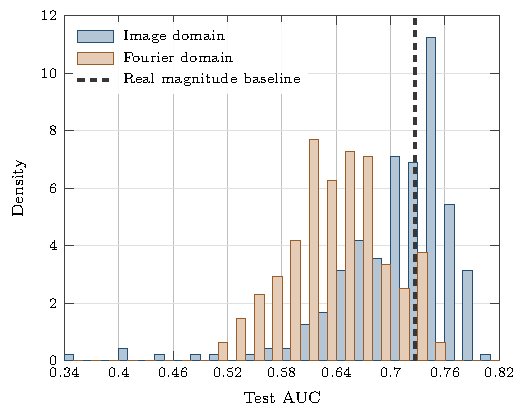
\includegraphics[width=\columnwidth]{../figures/results_auc_landscape/figure_auc_landscape_artwork.pdf}
\caption{Distribution of test AUC across the 480 complex-valued configurations. Image-domain and Fourier-domain configurations are shown using identical histogram bins; the dashed vertical line denotes the fixed real magnitude baseline.}
\label{fig:auc-landscape}
\end{figure}

\subsection{Input-Domain Summary}
The real magnitude baseline achieved test AUC $0.7268$. The complex grid contains 480 configurations, split evenly between 240 image-domain and 240 Fourier-domain configurations. Image-domain complex models had mean AUC $0.7102$ and Fourier-domain complex models had mean AUC $0.6377$, giving the broadest observed separation between the two input domains. The matched domain comparison covers 240 architecture pairs; image-domain AUC exceeded Fourier-domain AUC in 196/240 pairs ($81.7\%$), with mean paired $\Delta$AUC (image minus Fourier) $+0.0725$ and median paired $\Delta$AUC $+0.0852$. These paired quantities, together with the Wilcoxon signed-rank statistic and rank-biserial effect size in the table, are descriptive properties of the finite factorial grid and are not interpreted as population-level inference.

\begingroup
\renewenvironment{table}{\begin{table*}}{\end{table*}}
% Requires: \usepackage{booktabs}

\begin{table}[t]
\centering
\small
\setlength{\tabcolsep}{3pt}
\caption{Descriptive summary of test AUC for the observed image-domain and Fourier-domain complex configurations. Percentages count configurations exceeding the fixed real magnitude baseline (AUC $=0.7268$).}
\label{tab:results_auc_landscape_summary}
\begin{tabular}{lrrrrrrrr}
\toprule
Domain & $n$ & Mean & SD & Median & IQR & Min & Max & $>$ baseline, $n$ (\%) \\
\midrule
Image   & 240 & 0.7102 & 0.0665 & 0.7251 & 0.0740 & 0.3464 & 0.8162 & 116 (48.3) \\
Fourier & 240 & 0.6377 & 0.0536 & 0.6384 & 0.0689 & 0.5037 & 0.7534 & 14  (5.8) \\
\bottomrule
\end{tabular}
\end{table}

\begin{table}[t]
\centering
\small
\setlength{\tabcolsep}{5pt}
\caption{Paired descriptive comparison of test AUC for matched image-domain and Fourier-domain configurations. Each pair holds pooling, normalization, convolution, activation, stream level, and interaction level fixed. The Wilcoxon signed-rank result and paired rank-biserial effect size are descriptive measures for the observed factorial pairs, not strong population inference.}
\label{tab:results_auc_landscape_separation}
\begin{tabular}{lr}
\toprule
Measure & Value \\
\midrule
Number of matched pairs & $240$ \\
Mean paired $\Delta$AUC (image $-$ Fourier) & $+0.0725$ \\
SD of paired $\Delta$AUC & $0.0877$ \\
Median paired $\Delta$AUC & $+0.0852$ \\
IQR of paired $\Delta$AUC & $0.1125$ \\
$\Delta$AUC $>0$, $n$ (\%) & $196$ (81.7) \\
Wilcoxon signed-rank statistic & $3471.5$ \\
Wilcoxon $p$-value (two-sided) & $1.86\times10^{-24}$ \\
Paired rank-biserial effect size & $+0.7599$ \\
\bottomrule
\end{tabular}
\end{table}

\endgroup

\subsection{Factor-Level Summaries and Selected Interactions}
The marginal factor table reports descriptive means across the finite complex grid; its $\Delta$ column is mean AUC at that factor level minus the overall complex-grid mean AUC. Normalization shows a visible marginal contrast, with complex BatchNorm higher than RMSNorm, whereas convolution and activation contrasts are comparatively smaller. The interaction table retains the implemented five-level combined stream/interaction factor (complex-only/none, complex-only/holographic, dual/none, dual/modulus gate, and dual/holographic) rather than treating stream and interaction as separate independent factors. The stream/interaction pattern depends on domain, while the image/Fourier domain contrast remains the largest broad marginal separation. These summaries are descriptive properties of the observed factorial grid and do not establish a universal operator ranking.

\begingroup
\renewenvironment{table}{\begin{table*}}{\end{table*}}
% Requires \usepackage{booktabs}.
\begin{table}[t]
\centering
\caption{Descriptive marginal factor-level summaries of test AUC over the 480 complex configurations. $\Delta$ denotes mean AUC minus the overall complex-grid mean.}
\label{tab:factor-effects-marginal}
\small
\begin{tabular}{llrrrrrr}
\toprule
Factor & Level & $n$ & Mean AUC & SD & Median & IQR & $\Delta$ \\
\midrule
Pooling & max & 160 & 0.671 & 0.077 & 0.674 & 0.096 & -0.003 \\
 & median & 160 & 0.673 & 0.070 & 0.673 & 0.110 & -0.001 \\
 & average & 160 & 0.678 & 0.063 & 0.679 & 0.099 & 0.004 \\
Normalization & RMSNorm & 240 & 0.663 & 0.076 & 0.666 & 0.113 & -0.011 \\
 & C-BatchNorm & 240 & 0.685 & 0.063 & 0.684 & 0.093 & 0.011 \\
Convolution & standard & 240 & 0.677 & 0.069 & 0.678 & 0.104 & 0.003 \\
 & widely linear & 240 & 0.671 & 0.072 & 0.673 & 0.109 & -0.003 \\
Activation & modReLU & 120 & 0.680 & 0.061 & 0.684 & 0.092 & 0.006 \\
 & Mag-SiLU & 120 & 0.671 & 0.069 & 0.666 & 0.111 & -0.003 \\
 & CReLU & 120 & 0.673 & 0.075 & 0.676 & 0.111 & -0.001 \\
 & cardioid & 120 & 0.671 & 0.076 & 0.673 & 0.103 & -0.003 \\
Stream/interaction & C-only / none & 96 & 0.672 & 0.068 & 0.676 & 0.087 & -0.002 \\
 & C-only / holo & 96 & 0.652 & 0.076 & 0.664 & 0.081 & -0.022 \\
 & Dual / none & 96 & 0.679 & 0.074 & 0.678 & 0.133 & 0.005 \\
 & Dual / gate & 96 & 0.690 & 0.058 & 0.703 & 0.086 & 0.016 \\
 & Dual / holo & 96 & 0.677 & 0.070 & 0.685 & 0.120 & 0.003 \\
\bottomrule
\end{tabular}
\end{table}

% Requires \usepackage{booktabs}.
\begin{table}[t]
\centering
\caption{Descriptive domain-by-factor interaction summaries of test AUC. Each cell averages over the remaining factorial dimensions.}
\label{tab:factor-effects-interactions}
\small
\begin{tabular}{llrrrrr}
\toprule
Domain & Level & $n$ & Mean AUC & SD & Median & IQR \\
\midrule
\multicolumn{7}{l}{\textit{Domain $\times$ normalization}} \\
Image & RMSNorm & 120 & 0.695 & 0.079 & 0.714 & 0.086 \\
 & C-BatchNorm & 120 & 0.725 & 0.046 & 0.734 & 0.056 \\
Fourier & RMSNorm & 120 & 0.631 & 0.056 & 0.623 & 0.075 \\
 & C-BatchNorm & 120 & 0.645 & 0.050 & 0.648 & 0.058 \\
\midrule
\multicolumn{7}{l}{\textit{Domain $\times$ stream/interaction}} \\
Image & C-only / none & 48 & 0.682 & 0.079 & 0.690 & 0.093 \\
 & C-only / holo & 48 & 0.670 & 0.087 & 0.681 & 0.060 \\
 & Dual / none & 48 & 0.741 & 0.033 & 0.748 & 0.032 \\
 & Dual / gate & 48 & 0.725 & 0.044 & 0.732 & 0.048 \\
 & Dual / holo & 48 & 0.734 & 0.039 & 0.740 & 0.050 \\
Fourier & C-only / none & 48 & 0.662 & 0.055 & 0.660 & 0.082 \\
 & C-only / holo & 48 & 0.634 & 0.059 & 0.638 & 0.067 \\
 & Dual / none & 48 & 0.617 & 0.045 & 0.615 & 0.070 \\
 & Dual / gate & 48 & 0.656 & 0.050 & 0.656 & 0.077 \\
 & Dual / holo & 48 & 0.620 & 0.044 & 0.619 & 0.053 \\
\bottomrule
\end{tabular}
\end{table}

\endgroup

\subsection{Canonical Pooling Ablation}
The canonical comparison fixes image-domain input, ComplexRMSNorm2d (RMSNorm), standard complex convolution, a complex-only stream, no interaction, and modReLU. The three complex configurations differ only in the complex pooling operator: canonical max-pool, canonical median-pool, and canonical average-pool. Table~\ref{tab:canonical-comparison} reports these configurations together with the fixed real magnitude baseline for direct comparison.

\begingroup
\renewenvironment{table}{\begin{table*}}{\end{table*}}
\input{../tables/canonical_comparison/canonical_comparison.tex}
\endgroup

\subsection{High-Performing Configurations}
The maximum observed factorial AUC was \BestAUC with AP \BestAP for configuration \texttt{\BestLabel}. This is an exploratory maximum over the fixed 480-configuration grid evaluated on the same held-out test cohort, not an unbiased estimate of a selected final architecture.

\subsection{Joint AUC--AP Landscape}

Across the finite 480-configuration factorial grid, 114/480 complex configurations (23.8\%) exceeded the real baseline in both AUC and AP. This occurred for 101/240 image-domain configurations (42.1\%) and 13/240 Fourier-domain configurations (5.4\%). Across all configurations, AUC and AP showed a Pearson correlation of $r=0.755$ and a Spearman rank correlation of $\rho=0.788$. These quadrant counts and correlations are descriptive properties of the observed finite factorial grid.

% =============================================================================
\section{Discussion}\label{sec:discussion}
% =============================================================================
The completed factorial experiment does not support a universal advantage for complex-valued networks. Most complex configurations do not exceed the fixed magnitude baseline, while a subset does. The central conclusion is therefore conditional: the usefulness of complex-valued processing depends on the coordinate representation and the architectural operators used. This heterogeneity is precisely why the study evaluates a parameter-matched factorial grid rather than a single real-versus-complex pair.

Input representation provides the largest broad contrast in the observed grid. Image-domain configurations had mean AUC 0.7102, compared with 0.6377 for Fourier-domain configurations. In the 240 matched architectural pairs, all other factorial choices are held fixed within each pair, and the image-domain result was higher in 196/240 pairs (81.7\%), with mean paired image-minus-Fourier $\Delta$AUC of +0.0725 and median $\Delta$AUC of +0.0852. These are descriptive properties of the finite factorial grid, not causal or population-level statistical effects. A direct Fourier-domain classifier may impose a less favorable locality and aggregation bias for this slice-level anatomical task, but this does not imply that Fourier-domain information is intrinsically inferior. The Fourier arm is an FFT-derived representation of the prepared, phase-aligned complex images rather than untouched scanner raw k-space.

Normalization shows a visible but context-dependent contrast. Complex BatchNorm has the higher marginal mean AUC in the observed grid (0.685 versus 0.663 for RMSNorm). Its covariance whitening and learned Cartesian affine transformation may interact more favorably with this network and training setup than the study-specific ComplexRMSNorm2d implementation. The former is a literature-established complex normalization family, whereas the latter is an implementation choice designed here around running complex power. The observed marginal difference therefore does not establish universal superiority for Complex BatchNorm.

Standard versus widely-linear convolution shows a comparatively modest marginal contrast (mean AUC 0.677 versus 0.671), and the activation means are also close relative to the domain separation. This does not make widely-linear processing or any activation family useless. The value of conjugate flexibility and of the nonlinearities depends on their interaction with representation domain, normalization, pooling, and stream architecture. The factorial results should consequently not be read as a universal ranking of convolution or activation operators.

The combined stream/interaction factor is likewise domain dependent. It is one implemented five-level factor---complex-only/none, complex-only/holographic, dual/none, dual/modulus gate, and dual/holographic---rather than two independent stream and interaction dimensions. For example, the image-domain dual/none level has mean AUC 0.741, whereas the corresponding Fourier-domain level has mean AUC 0.617. This contrast illustrates that an interaction or stream design cannot be assigned a domain-independent value from the present grid. The dual-stream architectures and their optional mechanisms should be interpreted together with the coordinate system in which they operate.

The canonical pooling comparison provides a clean local architectural check because the three complex configurations hold image-domain input, ComplexRMSNorm2d, standard complex convolution, a complex-only stream, no interaction, and modReLU fixed, varying only pooling. The canonical max-pool reached AUC approximately 0.7527, compared with approximately 0.7283 for canonical median-pool and 0.7156 for canonical average-pool; their AP values were 0.148, 0.100, and 0.112, respectively, versus 0.106 for the real baseline. Max pooling therefore performs best among these three canonical choices, but this local comparison does not establish universal superiority across the full factorial grid. The comparison also connects the observed pooling behavior to the phase-coherence terms in Eq.~\eqref{eq:complex-average-coherence} without isolating pooling from the broader grid context.

Average precision is important here because the test cohort contains approximately 5\% positive slices. Across the joint AUC--AP landscape, 114/480 complex configurations (23.8\%) exceeded the real baseline in both metrics; the corresponding counts were 101/240 (42.1\%) for image-domain configurations and 13/240 (5.4\%) for Fourier-domain configurations. AUC and AP were strongly related over the grid, with Pearson $r=0.755$ and Spearman $\rho=0.788$, but they are not interchangeable under this class imbalance: AUC summarizes ranking across false-positive rates, whereas AP is sensitive to the precision achieved among relatively rare positives. These counts and correlations describe the finite factorial grid and do not constitute significance tests or population inference.

The maximum observed AUC of 0.8162 remains useful as an exploratory description of the architecture surface, not as the principal claim of the study. All 480 configurations were evaluated on the same fixed held-out test cohort, and selecting the highest observed test AUC from that grid introduces model-selection optimism. Accordingly, 0.8162 is not an unbiased estimate of the generalization performance of a selected final architecture.

Several limitations bound the interpretation. Each reported architecture has one training realization at fixed seed 10383, so stochastic optimization variability is not quantified. The same test cohort, containing only 63 positive slices, is reused across the 480 complex evaluations; this supports a finite-grid comparison but not independent uncertainty estimates for architecture selection. Metrics are reported at the slice level even though slices within a patient are correlated. The task is a slice-level PI-RADS 3--5 versus PI-RADS 1--2 classification, where PI-RADS 3--5 denotes radiological suspicion rather than histopathologically proven clinically significant cancer, and it is not a patient-level diagnosis.

The real comparator is magnitude-only, so the experiment does not separately identify the value of retaining real-imaginary information from the value of complex algebra. An information-matched real-valued network receiving concatenated real and imaginary channels would separate these mechanisms more cleanly. The study also uses a prepared four-coil T2-weighted subset and an FFT-derived Fourier representation rather than untouched scanner raw k-space. T2-only scope does not represent a complete biparametric or multiparametric clinical prostate MRI assessment, where complementary diffusion information and patient-level aggregation can matter.

The factorial experiment therefore establishes a controlled characterization of where complex-valued neural processing helps or fails under matched scalar capacity, rather than a universal claim of complex-valued superiority. The usefulness of complex-valued modeling for prostate T2 MRI classification is conditional on the coordinate representation and the architectural operators used; confirming a selected architecture requires repeated training realizations, patient-level analysis, and independent validation.

% =============================================================================
\section{Conclusion}\label{sec:conclusion}
% =============================================================================
This study formulates complex-valued prostate MRI classification as a parameter-controlled architecture experiment. A fixed magnitude-only CNN is compared with 480 complex configurations spanning image/Fourier representation, pooling, normalization, convolution, activation, and stream/interaction design. The completed grid shows that complex-valued processing is not intrinsically superior to magnitude-only learning: only \ComplexWins/\ComplexTotal complex configurations exceed the real-baseline AUC of \RealAUC. At the same time, the grid contains configurations with substantially higher observed discrimination, and the factor summaries reveal strong dependence on how the complex information is represented and processed.

The main conclusion is therefore conditional. Retaining complex information creates a larger representational space, but useful performance depends on the inductive bias imposed by the network. The current fixed-seed, fixed-test-cohort experiment characterizes that architecture surface; confirmation of a selected architecture requires additional uncertainty analysis and independent validation.


% These appendices are intentionally modular so they can later be moved to a
% supplementary document or an expanded arXiv version without rewriting the
% main manuscript.
\appendices

\section*{Acknowledgment}
\textit{Funding sources, collaborators, institutional acknowledgments, and data-use acknowledgments to be completed before submission.}

\ifCLASSOPTIONcaptionsoff
  \newpage
\fi
\bibliographystyle{IEEEtran}
\bibliography{Bibliography}

\end{document}
